\documentclass[a4paper,12pt,twoside]{article}
\usepackage[T1]{fontenc}
\usepackage[utf8]{inputenc}
\usepackage{lmodern}
\usepackage[french]{babel}
\usepackage{url,csquotes}
\usepackage[hidelinks,hyperfootnotes=false]{hyperref}
\usepackage[titlepage,fancysections,pagenumber]{polytechnique}
\usepackage{multirow}
\usepackage{wrapfig}


\title{Shortest Paths on Surfaces\\ Geodesics in Heat}
\subtitle{INF555 Digital Representation\\ and Analysis of Shapes }
\author{Ruoqi \bsc{He} \& Chia-Man \bsc{Hung}}

\begin{document}

\maketitle

%%%%%%%%%%%%%%%%%%%%%%%%%%%%%%%%%%%%%%%%%%%%%%%%%%%%%%%%%%%%%%%%%%%%%%%%%%%%%%
\section{Introduction}

In this project we present the algorithm of a practical method for computing approximate shortest paths (geodesics) and our implementation on triangle meshes. This method of Heat Flow is based on \textit{Geodesics in Heat: A New Approach to Computing Distance Based on Heat Flow}, Crane [2013]. Results are mainly showed by pictures. The last part is dedicated to additional work, including the two boundary conditions, the case of multisource and a system of navigation represented by a walking man on surface.

%%%%%%%%%%%%%%%%%%%%%%%%%%%%%%%%%%%%%%%%%%%%%%%%%%%%%%%%%%%%%%%%%%%%%%%%%%%%%%
\section{Heat flow algorithm}

In this section we explain the Heat Flow algorithm used in this project. It determines the geodesic distance to a specified subset of a given domain. We describe it on a triangle mesh.

Notations: heat field $u$, vector field $X$, distance function $\phi$.

\subsection{First Step}
Integrate the heat field $\dot{u} = \Delta u$.

The heat $u$ of a point on a considered surface is a value between 0 and 1. Source has 1 as its value.

In other words, we solve $(id - t\Delta)u_t = u_0$ where $u_t$ is the heat field after a time step $t$ and $u_0$ is the initial heat field.

On a triangle mesh and in matrix form, we have $(A - tLc)u = u_0$ where $A$ is a diagonal matrix containing the vertex areas, $A^{-1}Lc$ is the discrete Laplacian matrix of a triangle mesh, and $u_0$ is a vector which has value 1 on sources and 0 otherwise. Remark that here $u_0$ should be multiplied at left by $A$. However, in the case of one point source, this does not affect the second step.


\subsection{Second Step}
Evaluate the vector field $X = -\nabla u / \left | \nabla u \right |$.

We are only interested in the direction of $\nabla u$ and not in its value. $X$ points to the opposite direction of the source.

On a triangle mesh, by using the formula given in the article, we calculate the vector field on every triangle.

\subsection{Third Step}

Solve the Poisson equation $\Delta \phi = \nabla \cdot X$.

If a distance function $\phi$ exists, $\nabla \phi$ should give us a unit vector on every point, pointing to the opposite directin of the source. We approximate such a distance function $\phi$ by minimizing $\int \left | \nabla \phi - X \right |^{2}$, which is equivalent to solving the Poisson equation $\Delta \phi = \nabla \cdot X$.

On a triangle mesh and in matrix form, we solve $Lc\phi = b$ where $b$ is the vector of divergences of the vector field $X$.

%\subsection{Navigation}

%We also implemented a navigation system, represented by a walking man. He is positioned on the surface of the mesh and moves toward a given source point. 

%A walking man's position is defined by barycentric coordinates of a triangle of the mesh. A walk function takes a distance as its argument and first applys on the triangle on which he is standing and then recursively calls itself at the next triangle he comes across, until walking the given distance or reaching the source.

%%%%%%%%%%%%%%%%%%%%%%%%%%%%%%%%%%%%%%%%%%%%%%%%%%%%%%%%%%%%%%%%%%%%%%%%%%%%%%
\section{Implementation}

\subsection{Environment}

We chose Unity to implement the heat method in order to better visualize the result. All codes are written in C\#, and the scene is built with Unity Editor. For the main problem, we use the library ALGLIB to do sparse matrix operations and to solve linear equations. In addition, we use the C5 Generic Collection Library for the priority queue implementation.

%We used the half-edge data structure to present triangle meshes.

\subsection{Mesh representation}

\begin{wrapfigure}{r}{0.5\textwidth}
	\centering
	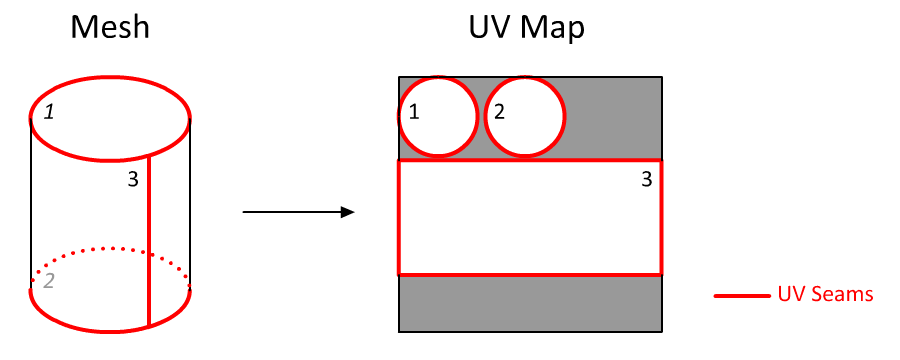
\includegraphics[width=0.5\textwidth]{F1.png}
	\caption{UV seams}
\end{wrapfigure}

We obtain ordinary triangle meshes via various ways. Those meshes are represented by a vertex array (array of Vector3) and a triangle array (sets of 3 indexes stored in an int array). We first wrote a method to convert them to half-edge representation, defined in Geometry.cs. The conversion can be done in time of $O(nd^2)$ where n is the number of vertices and d is the maximum degree of vertices. There are however two important things to consider:

\begin{wrapfigure}{l}{0.32\textwidth}
	\centering
	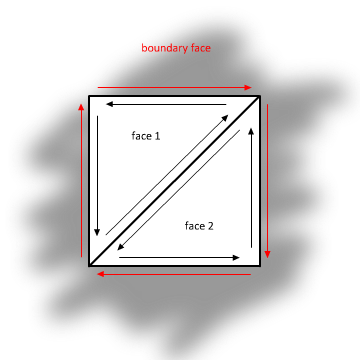
\includegraphics[width=0.32\textwidth]{F2.png}
	\caption{Boundary face}
\end{wrapfigure}

1. The half-edge representation is not well defined when using meshes with boundaries. In order to incorporate with other methods built on this representation, we decided to add a new face to cap each boundary. Those faces are marked as "boundary faces", and all vertices around them are marked as "boundary vertices". This way we can easily implement the boundary conditions in the heat method.

2. Many 3D models obtained from the internet have UV mappings, and thus have UV seams. This means that at the same position there can be two separate points having different UV coordinates. So the geometry we built may have seam-like boundaries blocking the way. To cope with this, we implemented a method to weld all overlapping vertices with a complexity of $O(nlogn)$, based on kdTree range searching.


\subsection{Matrix precalculation}

For each mesh loaded, we calculate in the first place its discrete unweighted laplacian matrix $-Lc$, and the matrices $A-tLc$ adapted to two different boundary conditions (if there are boundaries).

\begin{itemize}
\item
Dirichlet condition:

We set all elements in the rows/columns of the boundary vertices to 0, except the diagonal elements. This way the heat value will always be 0 at the boundary.

\item
Neumann condition:

The original laplacian matrix described in the paper satisfies Neumann condition.
\end{itemize}


We also build a Vector3 array of size (3 * triangle count) keeping all the values of cot(angle) * opposite edge vector, in order to accelerate the calculation of divergence.

For the first time, we skipped the Cholesky decomposition step since the overall performance without it is still reasonable. However, because of the numerical problems that we will explain afterwards, we finally implemented the Cholesky decomposition. It is applied on all precalculated matrices.

\subsection{Main calculation}

For single source problem, we follow these steps:

\begin{enumerate}
\item
Calculate the heat field $u$ by solving the heat equation $(A-tLc)u = u_0$.
\item
Calculate $X$, the normalized gradient of the heat field, on every triangle.
\item
Calculate $DivX$ on every vertex using the value of $X$ on its surrounding triangles.
\item
Calculate the distance field $\phi$ by solving the Poisson equation $Lc \phi = DivX$
\item
We then calculate the gradient of the distance field $\nabla \phi$ on every triangle which can be used to calculate the shortest paths.
\end{enumerate}

At first, without Cholesky decomposition, we used LinCG (Linear Conjugate Gradient) solver to solve linear equations. This solver solves symmetric positive-definite problems, but it works fine even with our second semi-definite problem (Poisson equation). We just need to shift the result such that the distance value at the source equals to zero.

\begin{wrapfigure}{r}{0.5\textwidth}
	\centering
	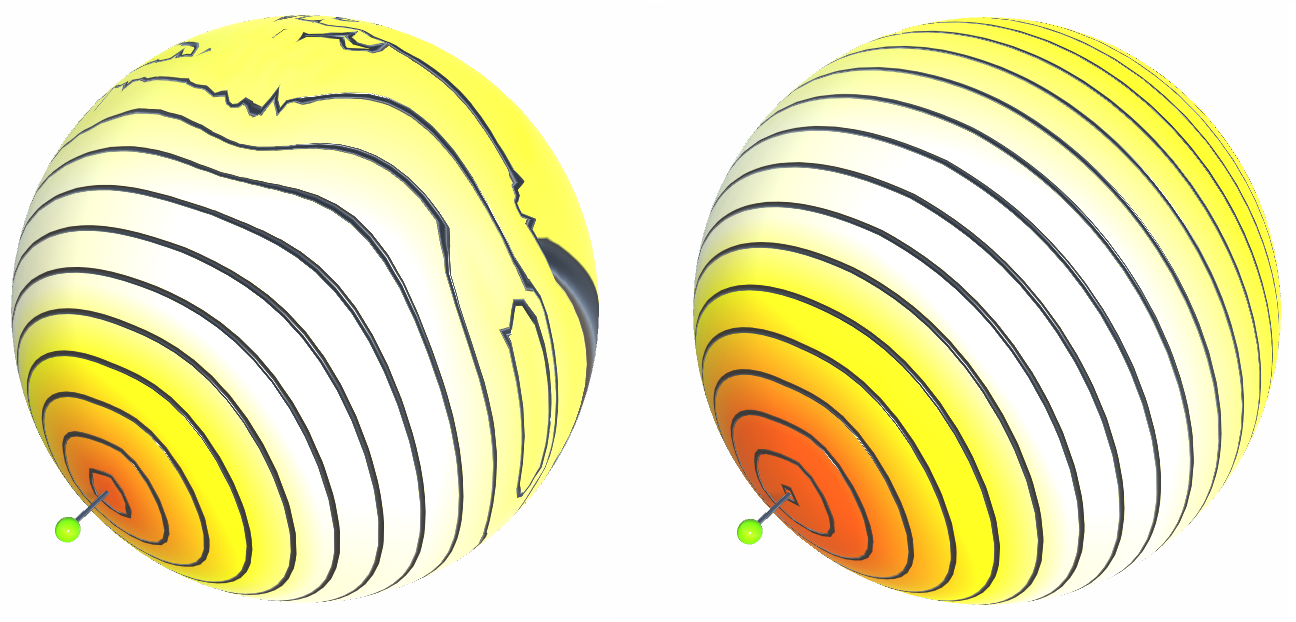
\includegraphics[width=0.5\textwidth]{P1.png}
	\caption{Left: LinCG / Right: Cholesky}
\end{wrapfigure}

%\begin{figure}[htb]
%	\centering
%	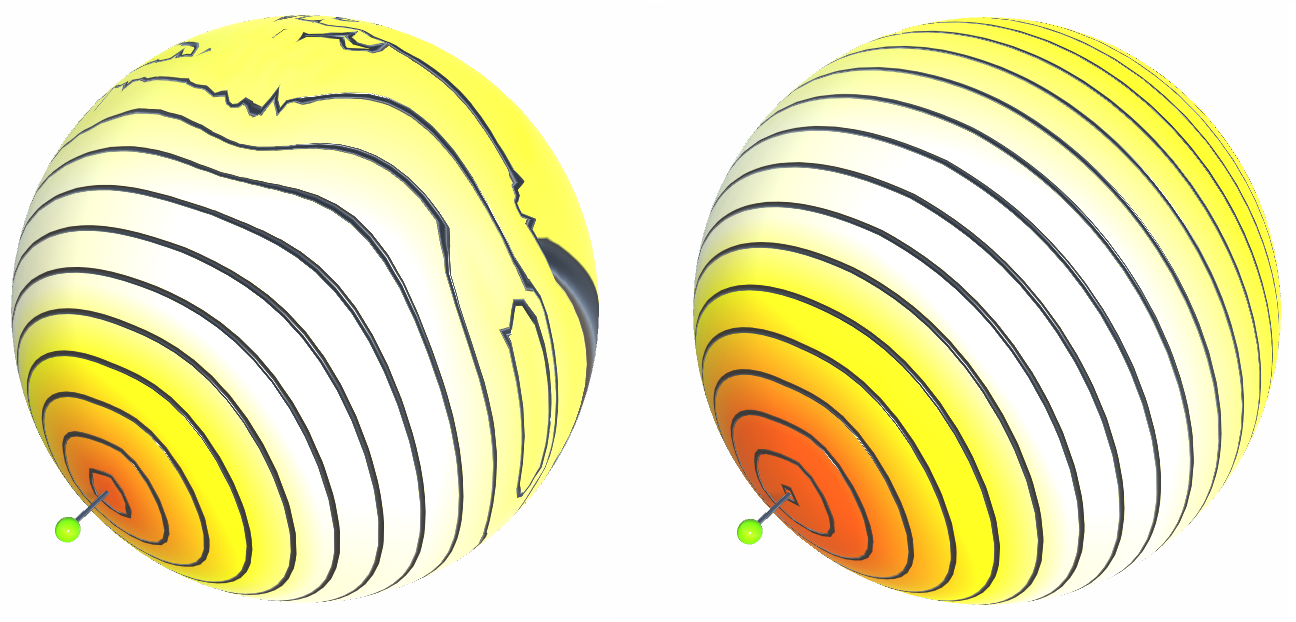
\includegraphics[width=0.8\textwidth]{P1.png}
%	\caption{P1}
%\end{figure}

However, from the result we obtained, we observed that LinCG solver is sensible to numerical errors. The solution of the heat equation contains values ranging from 1 to $10^{-20}$ or smaller. The longer the distance to the source, the smaller the heat value is. LinCG returns values of 0 when smaller than $\sim 10^{-12}$, so the heat gradient of the farther area cannot be computed. We can only improve the solution by increasing the time step $t$, which increases the heat value but creates a smoothed distance field.

Therefore, we chose to implement the Cholesky decomposition of matrices. It consists of decomposing a symmetric positive matrix $M$ into $LL^T$, where $L$ is a lower triangular matrix. This means the linear equation $LL^Tx = y$ becomes two basic triangular systems, that can be solved by simple substitution. This improves greatly the calculation time when switching sources (The decomposition is only calculated once for every mesh). And since we calculate the exact solution this way, we managed to have much smaller numerical errors, so as to eliminate the problems above. 
We overcame two difficulties regarding the Cholesky decomposition: 

\begin{itemize}
\item
While $M$ is a sparse matrix, $L$ is not necessarily sparse, especially when the entries of $M$ are mostly far away from the diagonal. This comes to one of our model which has randomly ordered vertices – it costs more than 4G RAM space to store the matrix $L$. After we reorder the vertices of the mesh along a certain axis, $L$ becomes much sparser and takes much less time to compute.
\item
We need to add a small regularization term to the diagonal entries of the laplacian matrix to get strict positive-definiteness (needed for the Cholesky decomposition of ALGLIB).
\end{itemize}

%%%%%%%%%%%%%%%%%%%%%%%%%%%%%%%%%%%%%%%%%%%%%%%%%%%%%%%%%%%%%%%%%%%%%%%%%%%%%%
\section{Results}

\subsection{Main results}

We successfully obtained some very nice results on a variety of meshes. Below are some pictures of the calculated geodesics and gradient fields.

\begin{figure}[htb]
	\centering
	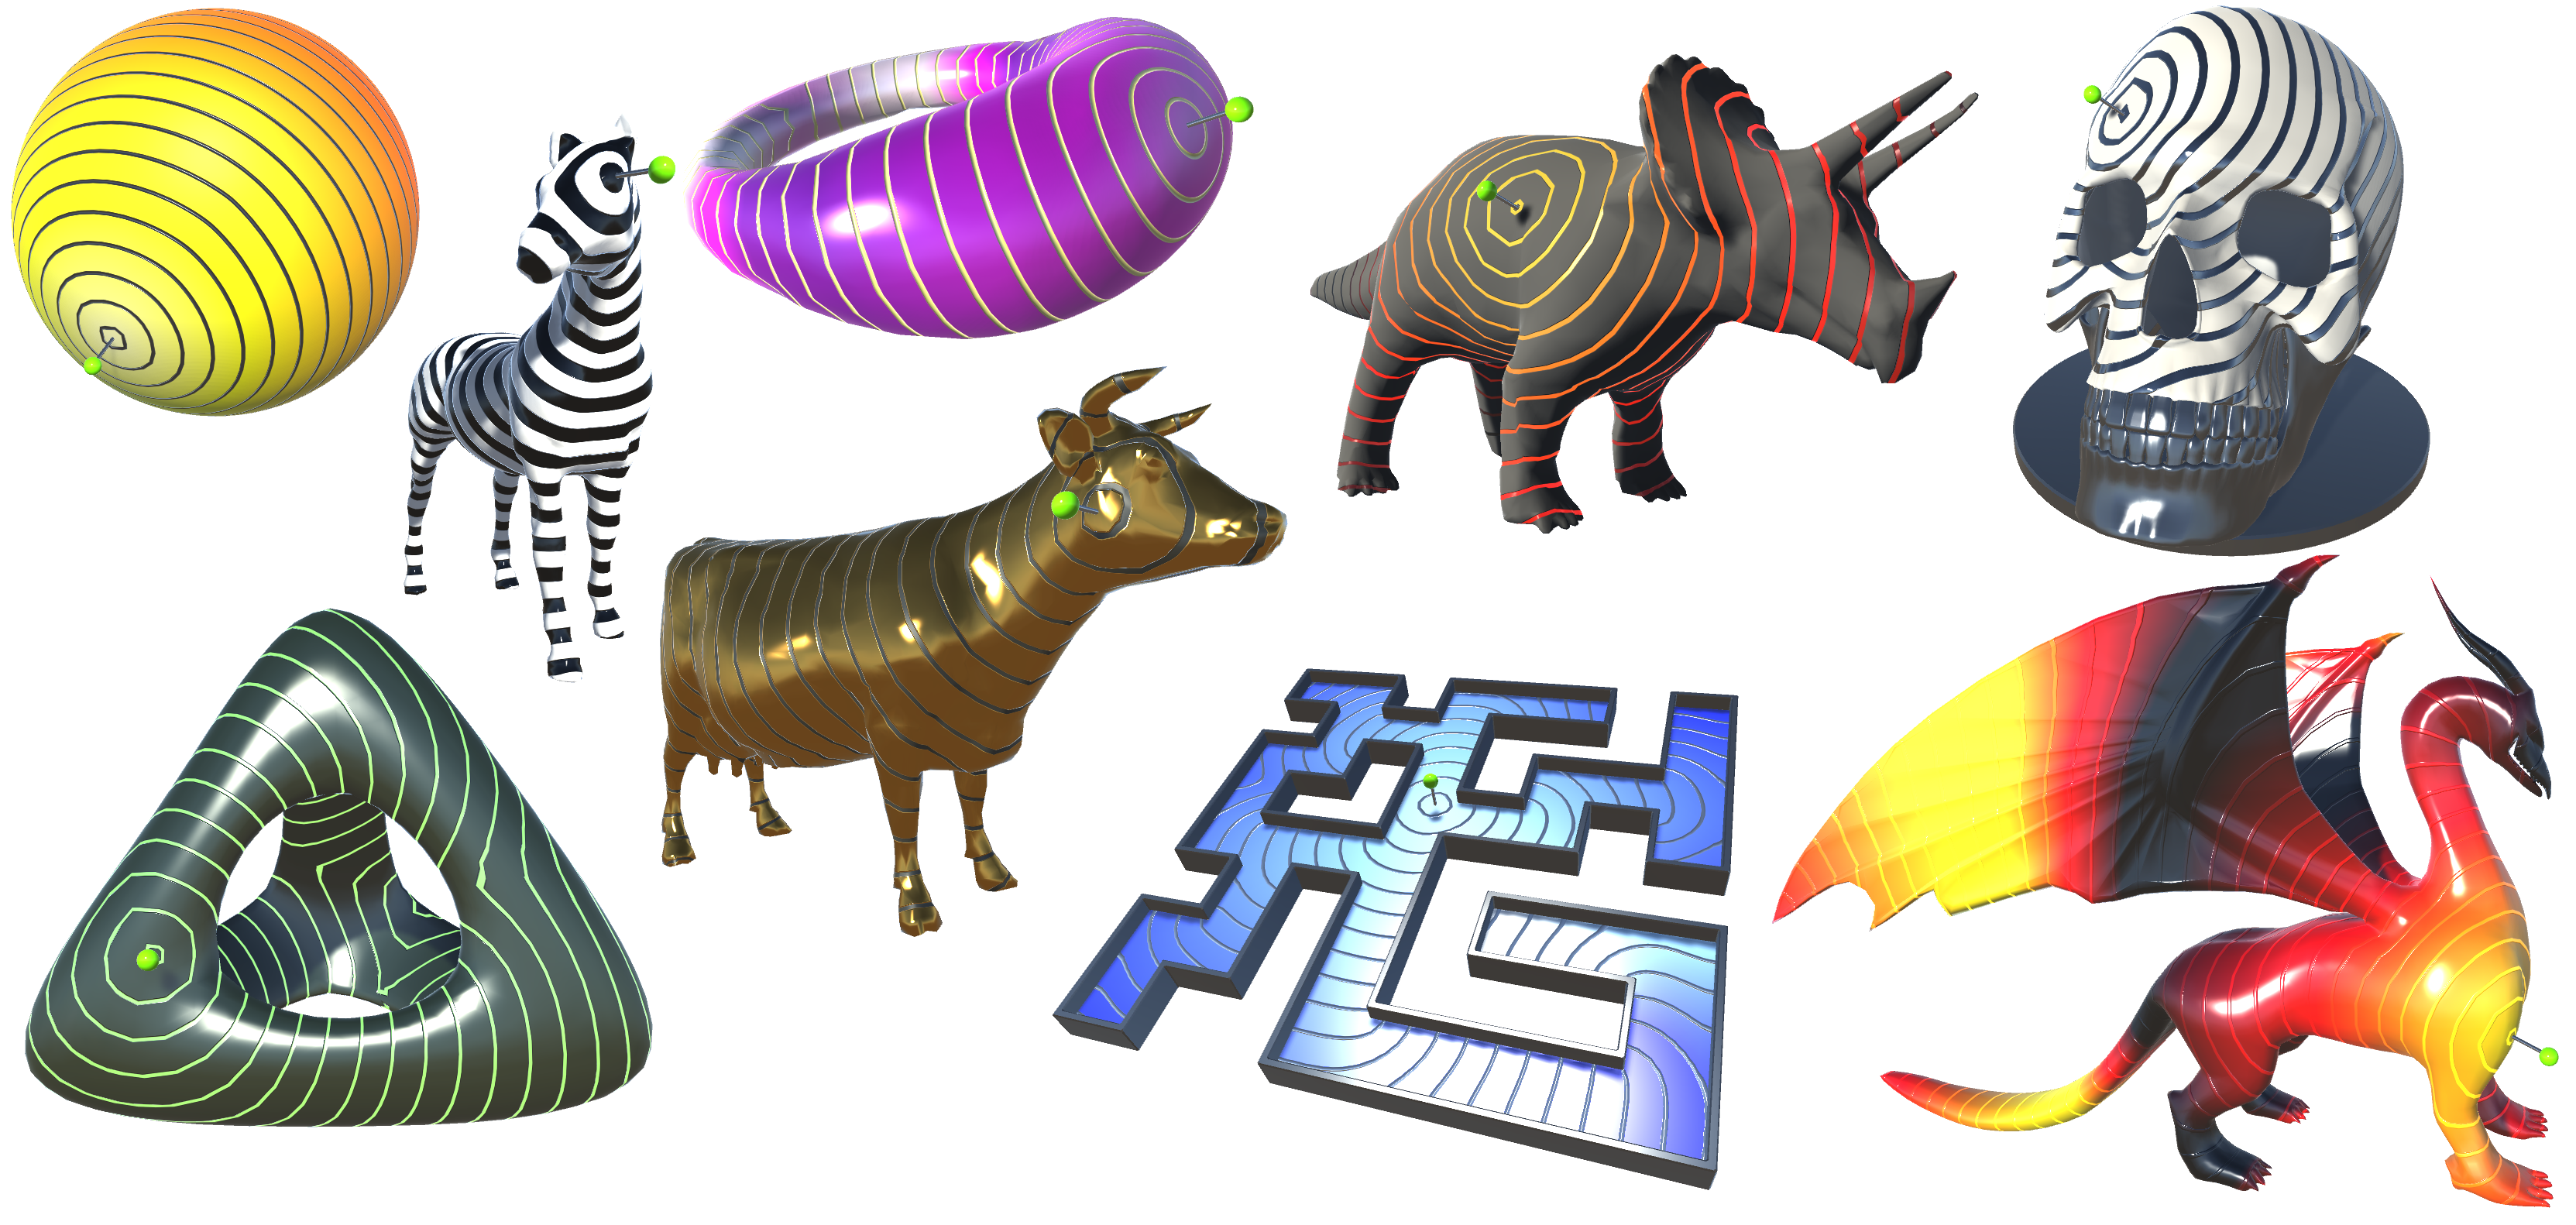
\includegraphics[width=\textwidth]{P4.png}
	\caption{Family photo}
\end{figure}

We observed the difference between the heat gradient and the distance gradient. The distance gradient smoothed out some non-uniform areas.

\begin{figure}[htb]
	\centering
	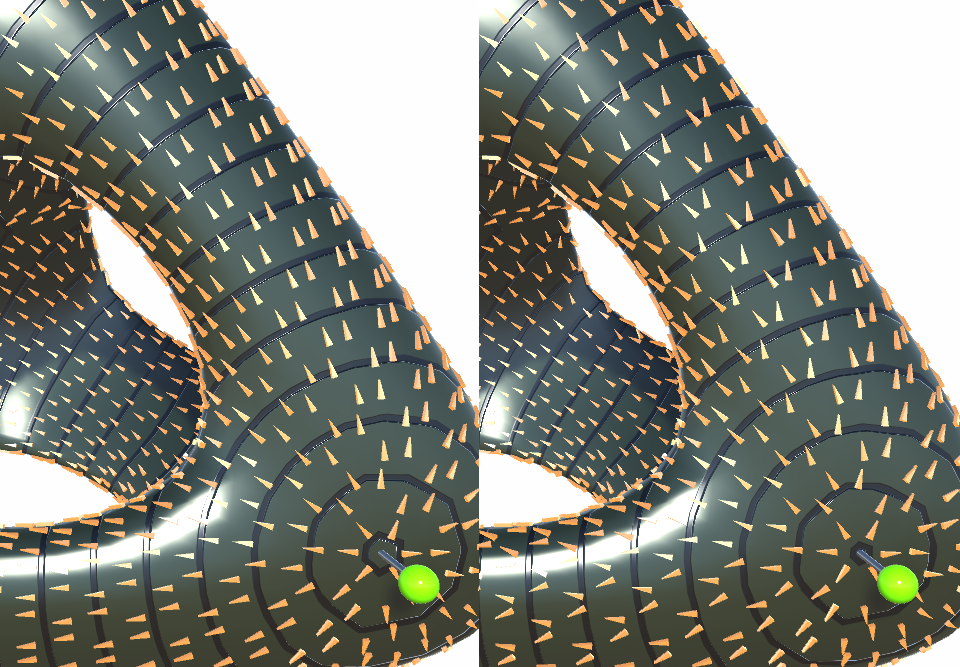
\includegraphics[width=0.5\textwidth]{P2.png}
	\caption{Left: Gradient of distance field/ Right: Gradient of heat field}
\end{figure}

%\begin{wrapfigure}{r}{0.3\textwidth}
%	\centering
%	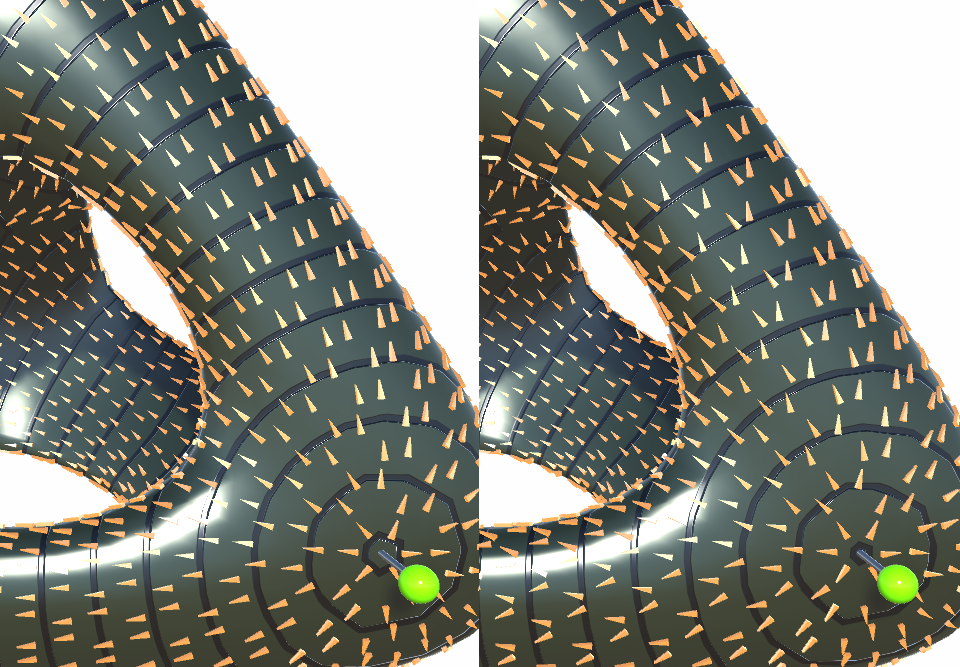
\includegraphics[width=0.3\textwidth]{P2.png}
%	\caption{P2}
%\end{wrapfigure}

\subsection{Time step t}

We usually set the time step t to the square of the maximum edge length. Using a much larger time step can create a smoothed distance. The smoothed distance is in general longer than the exact distance, because the trajectory is more curved. Below is an example of comparison.

\begin{figure}[htb]
	\centering
	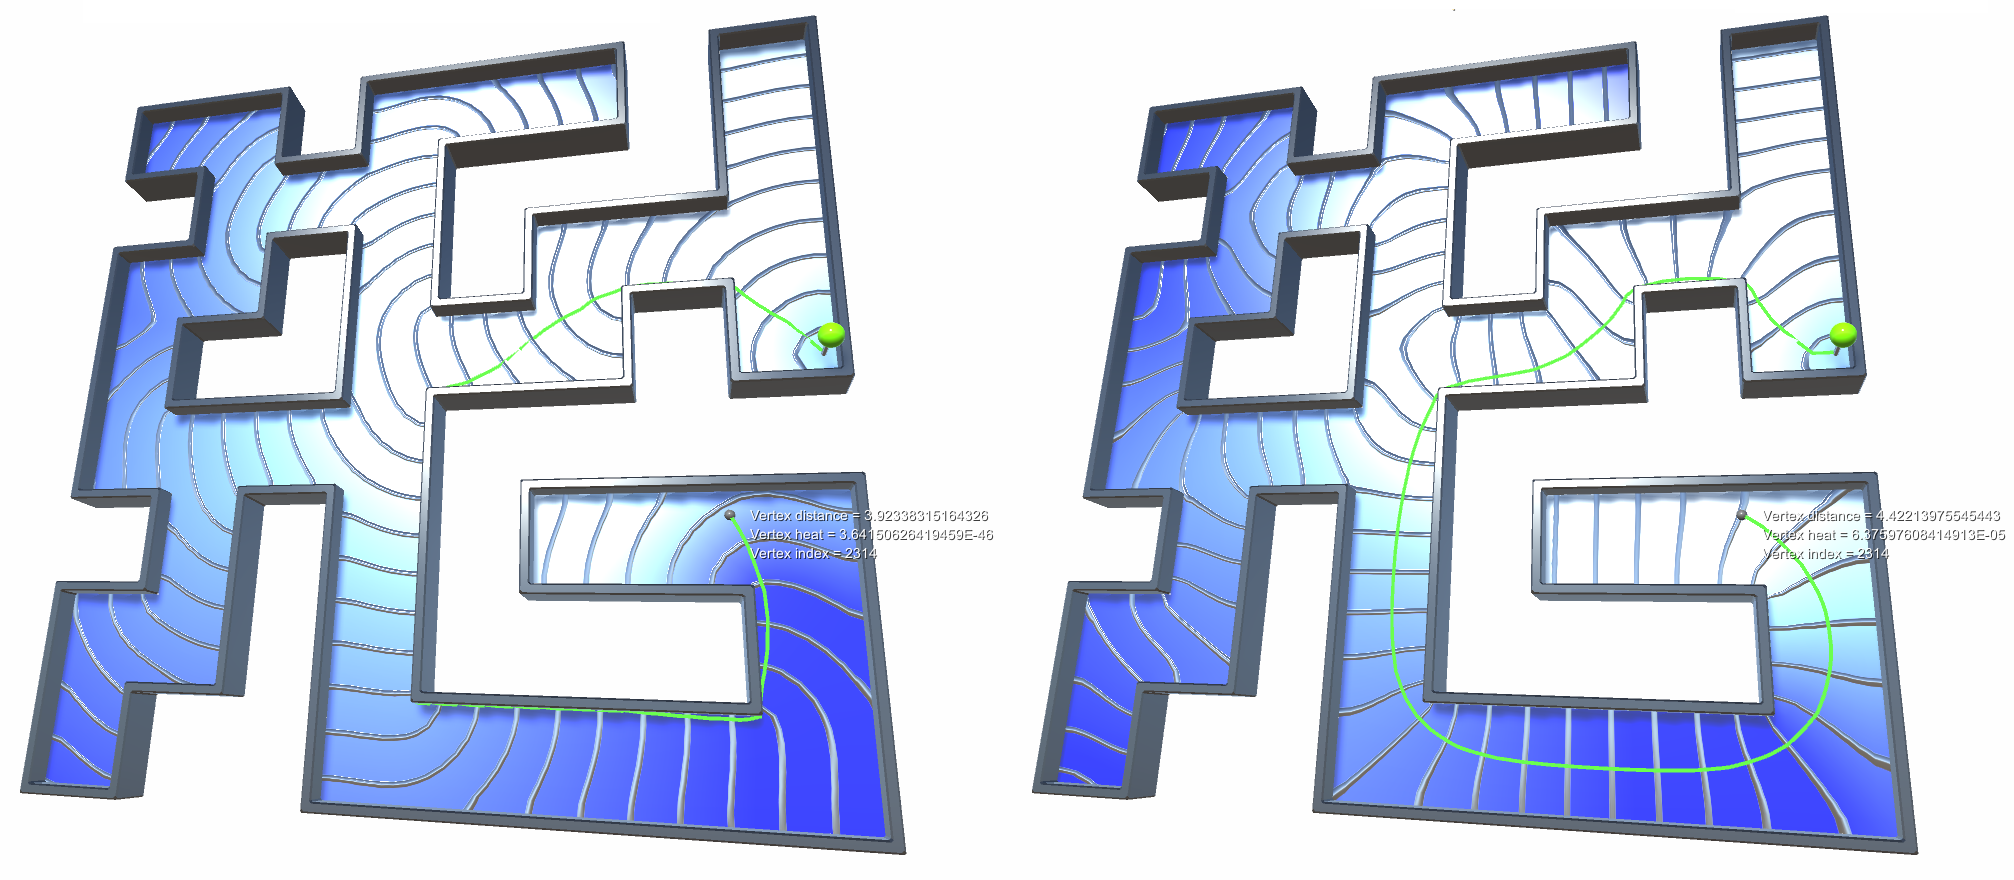
\includegraphics[width=0.8\textwidth]{P8.png}
	\caption{Left: $t=h^2$ / Right: $t=100h^2$ ($h$ is the maximum edge length)}
\end{figure}

%numerical error when $t = 1$ (choice of $t$), tweak parameter

\subsection{Boundary conditions}

We also compared the results when using different boundary conditions. We observed that with high value of $t$ (smoothed distance), the paths obtained tend to avoid borders with Dirichlet condition, and to adhere to borders with Neumann condition. And by using the average heat field calculated from two different conditions we get more natural paths.

\begin{figure}[htb]
	\centering
	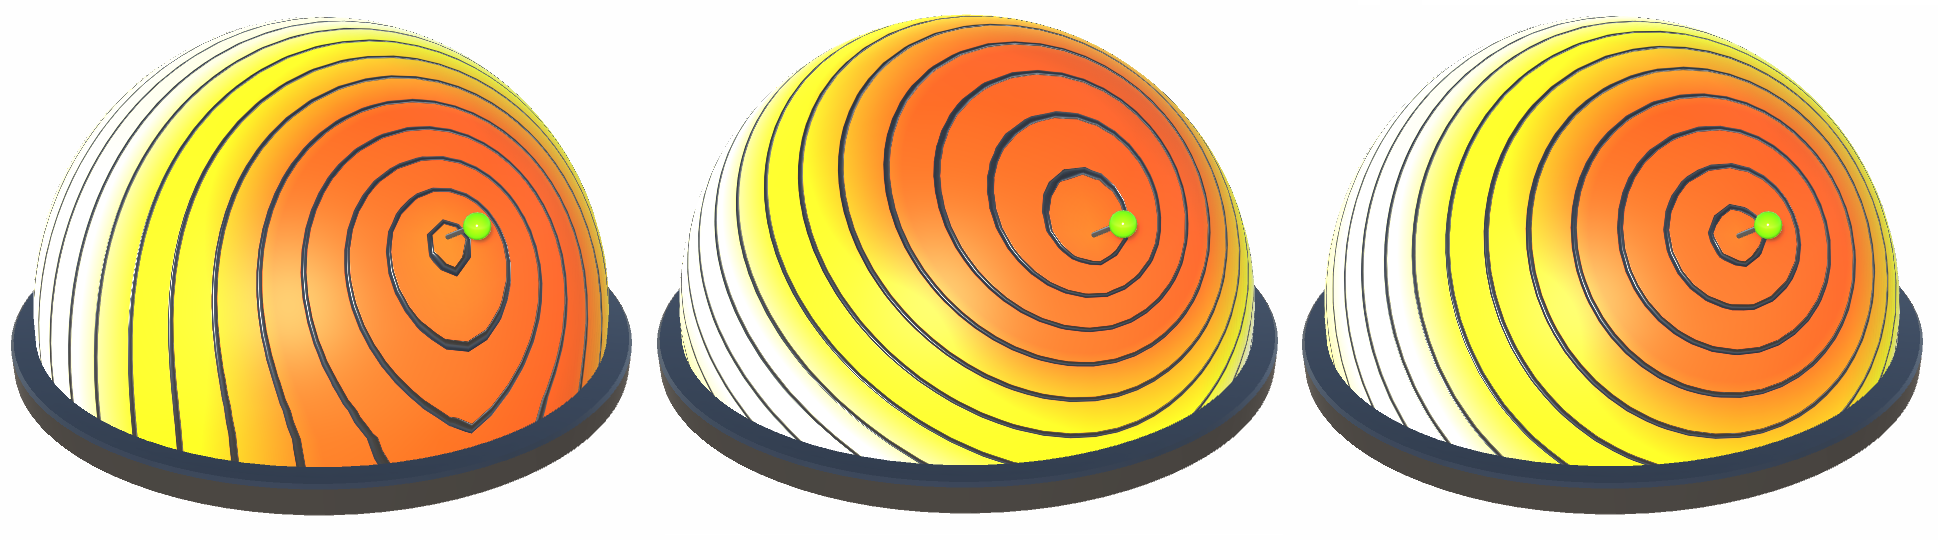
\includegraphics[width=0.8\textwidth]{P5.png}
	\caption{Left: Neumann / Middle: Dirichlet / Right: Average condition}
\end{figure}

\subsection{Broken mesh}

%\begin{wrapfigure}{r}{0.25\textwidth}
%	\centering
%	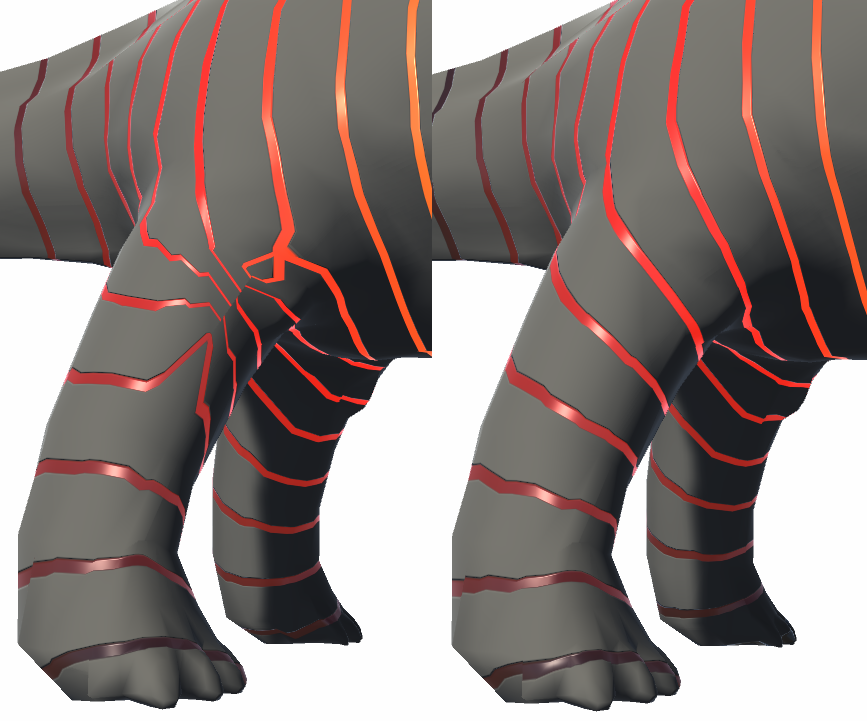
\includegraphics[width=0.25\textwidth]{P3.png}
%	\caption{P3}
%\end{wrapfigure}

The triceratops mesh that we tested has some bizarrely sharp obtuse triangles – they will break the positiveness of the heat matrix if we do not put a limit to the cotangent values of an angle. Even if we do, the result seems broken. We find a workaround by resetting the position of a vertex of the triangle to the average position of its neighbors.\\\\\\

\begin{figure}[htb]
	\centering
	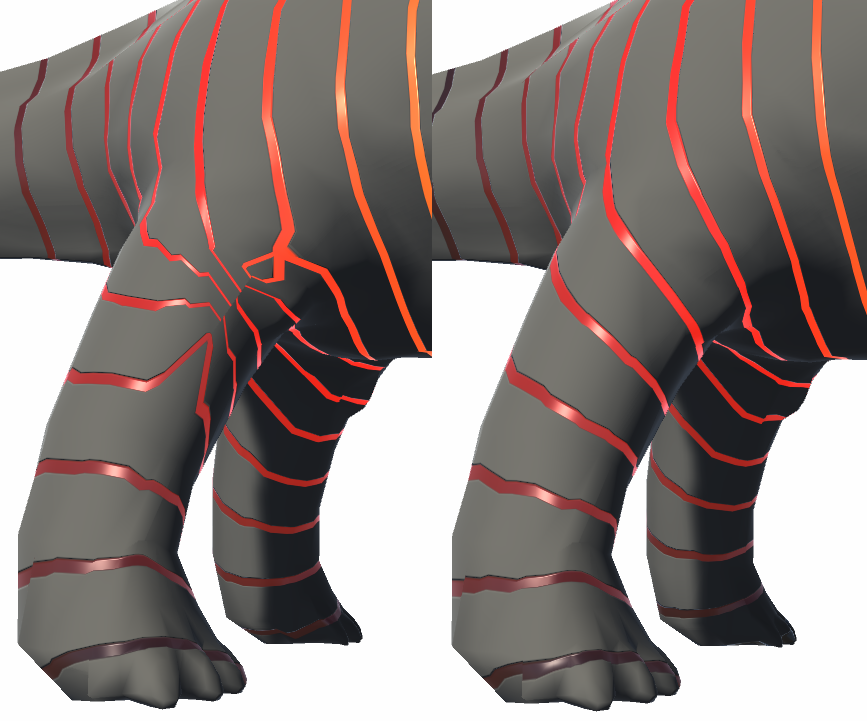
\includegraphics[width=0.34\textwidth]{P3.png}
	\caption{Mesh fixing}
\end{figure}

\subsection{Calculation time cost}

\begin{table}[htb]
\centering
\begin{tabular}{|c|c|c|c|c|c|c|}
  \hline
  
  %\multirow{2}{*}{Model} & \multirow{2}{*}{Triangles} & \multicolumn{2}{c|}{LinCG} & \multicolumn{2}{c|}{Cholesky} \\
  %& & Pre & Solve & Pre & Solve \\
  %\hline
  
  Model & Triangles & \multicolumn{2}{c|}{LinCG} & \multicolumn{2}{c|}{Cholesky} \\
  \cline{3-6}
  & & Pre & Solve & Pre & Solve \\
  \hline\hline
  
  High Genus & 3328 & 34ms & 27ms & 64ms & 8.9ms \\
  Bague & 5304 & 55ms & 60ms & 109ms & 17ms  \\
  Cow & 5804 & 62ms & 109ms & 335ms & 16ms \\
  Triceratops & 5660 & 59ms & 105ms & 306ms & 15ms \\
  Sphere 1 & 9024 & 94ms & 99ms & 236ms & 21ms \\
  Sphere 3 & 6912 & 65ms & 59ms & 327ms & 18ms \\
  Hemisphere & 3456 & 51ms & 34ms & 131ms & 10ms \\
  Skull & 12200 & 183ms & 338ms & 989ms & 38ms \\
  Maze & 5120 & 63ms & 94ms & 134ms & 12ms \\
  Horse & 39996 & 447ms & 1355ms & 2047ms & 113ms \\
  Dragon & 20388 & 188ms & 1291ms & 1787ms & 58ms \\
  \hline
\end{tabular}
\caption{Comparison of LinCG and Cholesky decomposition}
\end{table}

%\phantom \\

\section{Additional work}

\subsection{How we obtain meshes?}
Below are the four options we used:

\begin{enumerate}

\item
OFF format mesh from TD (High Genus, Bague, Cow, Triceratops, Horse) -> Unity mesh -> halfedge mesh

We wrote a OFF parser to transform OFF format meshes into Unity meshes.

\item
Internet resources (Skull, Dragon) -> Unity mesh -> processing (weld uv seams) -> halfedge mesh

\item
3Dmax handmade mesh (Maze, Sphere 2 \& 3, Hemisphere) -> Unity mesh -> halfedge mesh

\item
Code generated mesh (Sphere 1) -> halfedge mesh

\end{enumerate}

\subsection{Optimization}
Our solver ALGLIB solves sparse symetric positve-definite matrix system a lot faster than only symetric matrix system and Cholesky decomposition works only with symetric positve-definite matrix.
We noticed that $-Lc$ is a symetric positve-semidefinite matrix.
Therefore, $A-tLc$ (for $t>0$) in the first step is a symetric positve-definite matrix and $\epsilon I-Lc$ (for $\epsilon >0$) in the third step is also a symetric positve-definite matrix. Below is a math proof.

Prove that $-Lc$ is a symetric positve-semidefinite matrix.

We note $U_{ij}=E_{ii}+E_{jj}-E_{ij}-E_{ji}$ where $E_{ij}$ is an elementary matrix with only one nonnull value $1$ on position $(i,j)$. By definition, $-Lc$ is in form  $-Lc=\sum_{i,j}u_{ij}U_{ij}$ with all $u_{ij}>0$. Since the eigenvalues of $U_{ij}$ is $0$ and $2$, it is a symetric positve-semidefinite matrix. We conclude by saying that any positive combination of symetric positve-semidefinite matrices is also a symetric positve-semidefinite matrix. (Another proof is given in Lecture 9.)\\

\subsection{Multisource}

We also tried calculating the geodesics on surfaces when multiple vertices are marked as sources. However, by simply changing the initial heat vector to  $u_0$ (the vector which has value 1 on sources and 0 otherwise) we generate incorrect heat field and distance field – the solved heat field $u_t$ cannot guarantee equal values at each source vertex, and thus not every source vertex has a distance of zero. Typically, the vertex surrounded by more source vertices has a higher temperature and a negative distance.

\begin{figure}[htb]
	\centering
	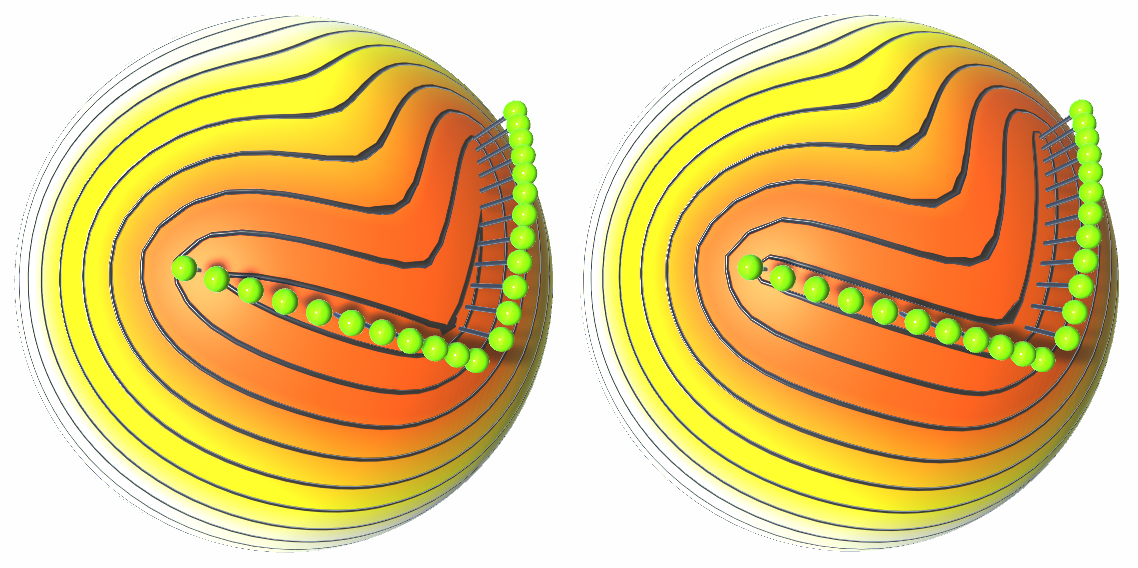
\includegraphics[width=0.6\textwidth]{P6.png}
	\caption{Left: Simply adding source on $u_0$ / Right: Accurate multisource}
\end{figure}

We solved this by imposing the constraints $u_t = 1$ at every source vertex in the heat equation, and also the constraint $\phi = 0$ at every source vertex in the Poisson equation. (The first constraint cannot imply the second since the distance field we get is only the closest potential of the heat gradient field.)

One downside, however, is that the matrices need to be modified to contain these extra constraints related to the source. For exemple, to have $u_t = 1$ at the source we put $1$ at the diagonal entries of the sources, and $0$ everywhere else in the same lines and columns. We then compensate the terms we deleted by adding an additional vector at the right side of the equation. Because of this, the Cholesky decomposition need to be carried out each time we change the source. This slows down the calculation a lot.

\subsection{Navigation}

\begin{wrapfigure}{r}{0.36\textwidth}
	\centering
	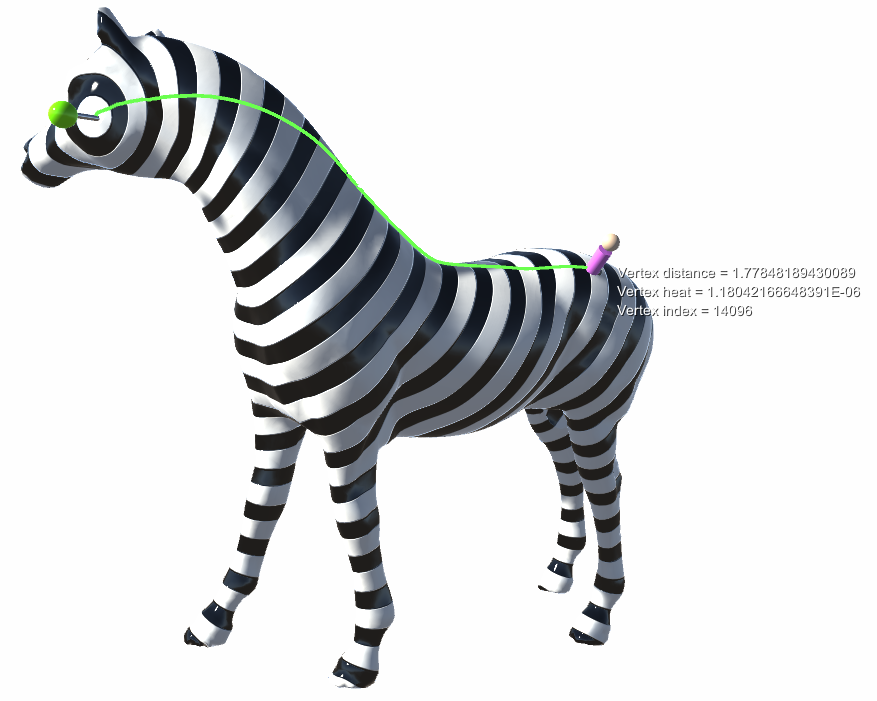
\includegraphics[width=0.36\textwidth]{P7.png}
	\caption{Navigation}
\end{wrapfigure}

Now that we have the distance field, we would like to calculate the path from a given point to the source point. We achieved this by first calculating the gradient of the distance field (step 5 of the main calculation) which is considered uniform on every triangle, then tracing a trajectory by recursively following the gradient in every triangle and entering the next one.

We visualized this process by moving a walking man on the surface of the mesh. His position is defined by barycentric coordinates of the triangle he is standing on. The distance gradient on it is also converted to barycentric coordinates, but with a sum of 0. (In this way, we can add it to the position coordinates and still get a barycentric coordinate with a sum of 1.) A walk function takes a distance as its argument and first moves on the triangle on which he is standing. By finding the first coordinate that reaches zero we find the edge the man will come across. It then recursively calls itself at the next triangle he enters, until walking the given distance or reaching the source.


There are however two extra cases to consider:
\begin{itemize}
\item
The gradient is pointing to a boundary. In this case, when reaching a boundary, we walk alongside it towards the smaller-distance vertex.
\item
Two neighboring triangles have opposing gradient. In this case, when reaching the middle edge, we choose to follow the edge instead.
\end{itemize}

\subsection{Mapping}

In order to better visualize the distance field, we chose to map a striped texture onto the surface of the mesh. It is actually quite simple: We create some striped textures with color gradient that are only one pixel tall, assign it to the mesh, and for each vertex we set the U value of its UV coordinates to its distance to the source. And that’s it! When rendering the texture, each point on a triangle has its U coordinate interpolated from the three vertices of the triangle, and it is exactly the interpolated distance of this point – so it will be colored by the pixel of the striped texture representing this distance.
To make it even better, in addition to the main texture, we also apply generated normal map, specular map and emission map to each model, making it especially realistic. We just need to set the tangent vector of each vertex to the average distance gradient on it to make the normal map work.

\begin{figure}[htb]
	\centering
	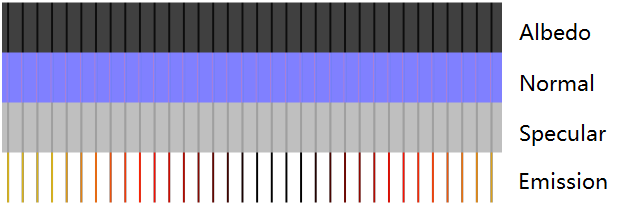
\includegraphics[width=0.6\textwidth]{P9.png}
	\caption{An example of generated textures}
\end{figure}

%Albedo, Normal, Specular Smoothness, Emission

\subsection{Dijkstra}
We implemented a simple Dijkstra shortest path algorithm on the graph made by the vertices and edges of the mesh. This allows us to easily create a line of source vertices connecting two selected vertices. (In the demo, press shift and click on the surface of the mesh.)


%%%%%%%%%%%%%%%%%%%%%%%%%%%%%%%%%%%%%%%%%%%%%%%%%%%%%%%%%%%%%%%%%%%%%%%%%%%%%%
\section{Conclusion \& extensions}
Path finding is an important topic and has applications in several domains, such as video games and robotics. The heat method is a simple way that allows us to compute approximate geodesics to a point source or a specific domain of source (multisource) efficiently. In this project we succeeded to implement this method on surfaces represented by triangle meshes. A system of navigation is added to visualize the shortest path taken. Some extra work is done to improve the visualization, such as texture mappings.

Regarding improvement we could make, in the case of multisource repeated calculation of Cholesky decomposition is required due to the constraints of multisources. It might be possible to operate on the Cholesky decomposition of $Lc$ to cleverly avoid recalculating the decomposition each time we change the source.

One extension we can think of is adding different weight on different areas to represent the difficulty of passing through. Another is changing the form of the considered domain from surfaces represented by triangle meshes to bounded spaces represented by tetrehedron meshes.


\end{document}